\documentclass[hyperref={pdfpagelabels=false}]{beamer}
\usepackage[ngerman]{babel}
\usepackage[utf8]{inputenc}
\usepackage{multicol}
\usepackage{csquotes}


%\usepackage{lmodern}

\title{Thema 10: Continuous Integration und Jenkins}   
%\subtitle{Skalierbare verteilte Datenanalyse}
\author{Daniel Wolfschmidt} 
\date{02.09.2018} 

\usetheme{Malmoe}

\usepackage{beamerthemeshadow}


\useoutertheme{infolines}

%  \beamersetuncovermixins{\opaqueness<1>{25}}{\opaqueness<2->{15}}
%  sorgt dafuer das die Elemente die erst noch (zukuenftig) kommen 
%  nur schwach angedeutet erscheinen 
\beamersetuncovermixins{\opaqueness<1>{25}}{\opaqueness<2->{15}}
% klappt auch bei Tabellen, wenn teTeX verwendet wird\ldots



%NO FOOTLINE
%gets rid of bottom navigation bars
%\setbeamertemplate{footline}[frame number]{}

%gets rid of bottom navigation symbols
\setbeamertemplate{navigation symbols}{}

%gets rid of footer
%will override 'frame number' instruction above
%comment out to revert to previous/default definitions
\setbeamertemplate{footline}{}

\setbeamercovered{transparent}

%\setbeamertemplate{frametitle}{\nointerlineskip  
 %   \begin{beamercolorbox}[wd=\paperwidth,ht=2.75ex,dp=1.375ex]{frametitle}
  %      \hspace*{2ex}\insertframetitle \hfill {\insertframenumber} \hspace*{1ex}%
   % \end{beamercolorbox}}

%\addtobeamertemplate{headline}{}{\rule{\paperwidth}{3pt}}

\setbeamercolor{mycolor}{fg=blue,bg=blue}

\addtobeamertemplate{headline} 
{
  \leavevmode%
  \hbox{%
  \begin{beamercolorbox}[wd=.333333\paperwidth,ht=2.25ex,dp=1ex,center]{mycolor author in head/foot}%
    Daniel Wolfschmidt
		%\usebeamerfont{author in head/foot}\insertsection
  \end{beamercolorbox}%
  \begin{beamercolorbox}[wd=.333333\paperwidth,ht=2.25ex,dp=1ex,center]{mycolor title in head/foot}%
   
		Continuous Integration und Jenkins		
  \end{beamercolorbox}%
  \begin{beamercolorbox}[wd=.333333\paperwidth,ht=2.25ex,dp=1ex,right]{mycolor date in head/foot}%
    \usebeamerfont{date in head/foot}\insertshortdate{}\hspace*{2em}
    \insertframenumber{} / \inserttotalframenumber \hspace*{2ex} 
  \end{beamercolorbox}}%
  \vskip0pt%
}


\begin{document}




\begin{frame}[plain,noframenumbering]
\titlepage
\end{frame} 


\begin{frame}
\frametitle{Inhaltsverzeichnis}
\setcounter{tocdepth}{1}
\tableofcontents
\end{frame} 





\section{} 
\begin{frame}
\frametitle{} 
\begin{center}
\textit{\LARGE{”The most powerful tool we have as developers is automation“}}
\end{center}
\vspace{0.5cm} 
\begin{flushright}
\footnotesize{Scott Hanselman\\ Programmer, teacher and speaker\\ Microsoft Web Platform Team}
\end{flushright}

\end{frame}


\section*{Einleitung} 
\begin{frame}[t]
\frametitle{Einleitung} 

Heutige Probleme:
\begin{itemize}
\item  Immer schnellere Entwicklungszyklen 
\item  Punkt2
\item  Punkt3
\item  Punkt4
\end{itemize}  


\visible<2-> { \huge{Deshalb CI einführen!}  }

\end{frame}
\section{Continuous Integration} 
\begin{frame} [t]
\frametitle{Continuous Integration} 

Ablauf dieses Teiles
\begin{itemize}
	\item Begriffsklärung und Abgrenzung zu ähnlichen Begriffen
	\item Ablauf von Continuous Integration
	\item Gründe für den Einsatz von Continuous Integration	
	\item Mögliche Verbesserungen	
\end{itemize}

\end{frame}

\subsection{Begriffsklärung I}
\begin{frame} [t]
\frametitle{CI nach Martin Fowler}
\visible<1-> {
\begin{center}
\textit{”Continuous Integration is a software development practice where members of a team integrate their
work frequently, usually each person integrates at least daily - leading to multiple integrations per day.
Each integration is verified by an automated build (including test) to detect integration errors as
quickly as possible“}
\end{center}
\vspace{0.5cm} 
\begin{flushright}
\footnotesize{Martin Fowler\\ Geistiger Vater von CI\\ Thoughtworks}
\end{flushright}
}
\visible<2-> {
\vspace{0.5cm} 
\begin{multicols}{2}
\begin{itemize}
	\item kollaborativ
	\item häufiges Integrieren
	\item Nachweis des Erfolgs
	\item Automatisierung von Schritten
\end{itemize}
\end{multicols}
}
\end{frame}

\subsection{Begriffsklärung II}
\begin{frame} [t]
\frametitle{CI nach R.Owen Rogers}
\visible<1-> {
\begin{center}
\textit{”The practice of continuous integration represents a fundamental shift in the process of building software. It takes integration, commonly
an infrequent and painful exercise, and makes it a simple, core part of a developer’s daily activities. Integrating continuously makes integration a part of the natural rhythm of coding, an integral part of the test-code-refactor cycle. Continuous integration is about progressing steadily forward by taking small steps.“}
\end{center}
\vspace{0.5cm} 
\begin{flushright}
\footnotesize{R. Owen Rogers\\ Entwickler und Konferenzsprecher\\ Thoughtworks}
\end{flushright}
}
\visible<2-> {
\vspace{0.5cm} 
\begin{multicols}{2}
\begin{itemize}
	\item Auswirkungen im Fokus
	\item "`Test-Code-Refactor"'
	\item Teamaspekt eher implizit
	\item Sichtweisen decken sich
\end{itemize}
\end{multicols}
}
\end{frame}

\subsection{Begriffsklärung III}
\begin{frame} [t]
\frametitle{Zusammenfassend}
\visible<1-> {
Continuous Integration ist eine Praxis in der Softwareentwicklung, bei der folgende Punkte von zentraler Bedeutung sind:
}
\vspace{0.5cm} 
\begin{itemize}
\visible<2-> {
	\item Regelmäßige Integration in eine gemeinsame Codebasis
}
\visible<3-> {
	\item \textbf{Automatisierter} Nachweis des Integrationserfolgs
}
\visible<4-> {
	\item \textbf{Automatisierte} Tests
}
\visible<5-> {
	\item Schnelle Feedback Zyklen
}
\end{itemize}
\end{frame}

\subsection{Abgrenzung zu anderen Begriffen I}
\begin{frame} [t]
\frametitle{Continuous Delivery}
\visible<1-> {
\begin{center}
\textit{”You achieve continuous delivery by continuously integrating the software done by the development team, building executables, and running automated tests on those executables to detect problems.\\ Furthermore you push the executables into increasingly production-like environments to ensure the software will work in production. To do this you use a DeploymentPipeline.“}
\end{center}
\vspace{0.5cm} 
\begin{flushright}
\footnotesize{Martin Fowler\\ Geistiger Vater von CI\\ Thoughtworks}
\end{flushright}
}
\visible<2-> {
\vspace{0.5cm} 
\begin{multicols}{2}
\begin{itemize}
	\item Erweiterung von CI
	\item Schritte bis zum Kunden
	\item Auch umfangreichere Tests 
	\item Ziel ist rechtzeitig zu liefern
\end{itemize}
\end{multicols}
}
\end{frame}

\subsection{Abgrenzung zu anderen Begriffen II}
\begin{frame} [t]
\frametitle{Continuous Deployment}
\visible<1-> {
\begin{center}
\textit{”The concept of continuous deployment, i.e. the ability to deliver software functionality frequently to customers \textelp{}“}
\end{center}
\vspace{0.5cm} 
\begin{flushright}
\footnotesize{Helena Holmström Olsson\\ Dozentin für Computerwissenschaften\\ Universität Malmö}
\end{flushright}
}
\visible<2-> {
\vspace{0.5cm} 
\begin{multicols}{2}
\begin{itemize}
	\item Einen Schritt weiter als CD
	\item CD: Fester Lieferzeitpunkt
	\item Hier: Potentiell immer Lieferbar 
	\item Am weitesten Automatisiert
\end{itemize}
\end{multicols}
}
\end{frame}

\subsection{Abgrenzung zu anderen Begriffen III}
\begin{frame} [t]
\frametitle{Übersicht und Einordnung}
\begin{figure}[h]
  \centering
  \fbox{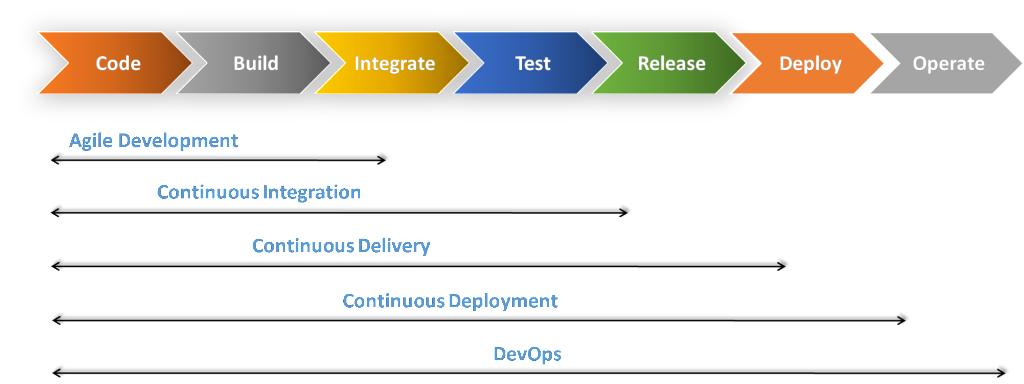
\includegraphics[width=110mm]{../Images/ci-cd-image-1024x384.png}}	  
\end{figure}
\end{frame}

\subsection{Ablauf von Continuous Integration}
\begin{frame} [t]
\frametitle{Ablauf nach Martin Fowler}
\begin{figure}[h]
  \centering
  \fbox{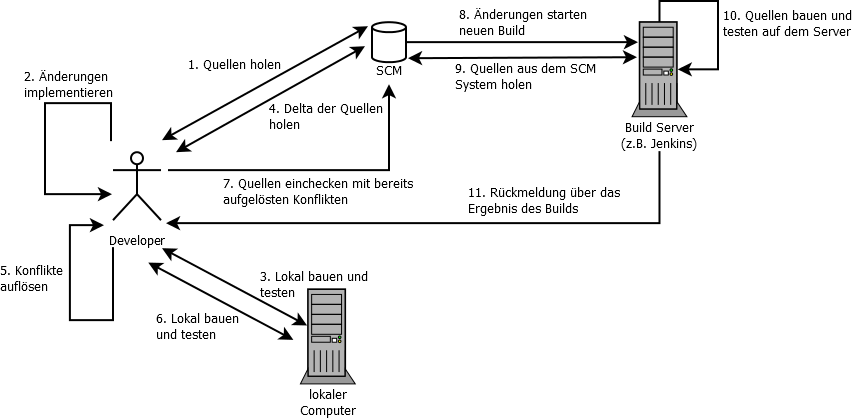
\includegraphics[width=110mm]{../Images/Schema-aufbau.png}}	  
\end{figure}
\vspace{0.5cm} 
Schematischer Ablauf von CI, wie er von Martin Fowler beschrieben wird
\end{frame}

\subsection{Ablauf nach Martin Fowler}
\begin{frame} [t]
\only<1>{
\frametitle{Baseline holen}
\begin{figure}[h]
  \centering
  \fbox{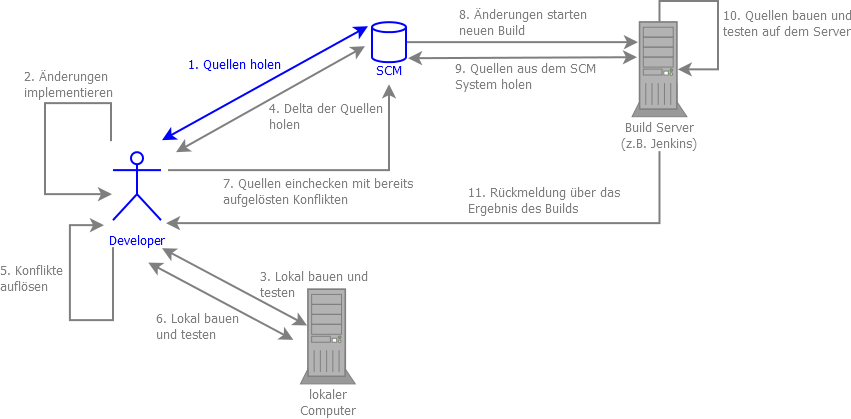
\includegraphics[width=110mm]{./Images/Schema-aufbau1.png}}	  
\end{figure}
\vspace{0.5cm} 
Entwickler holt sich Baseline
}
\only<2>{
\frametitle{Implementierung durchführen}
\begin{figure}[h]
  \centering
  \fbox{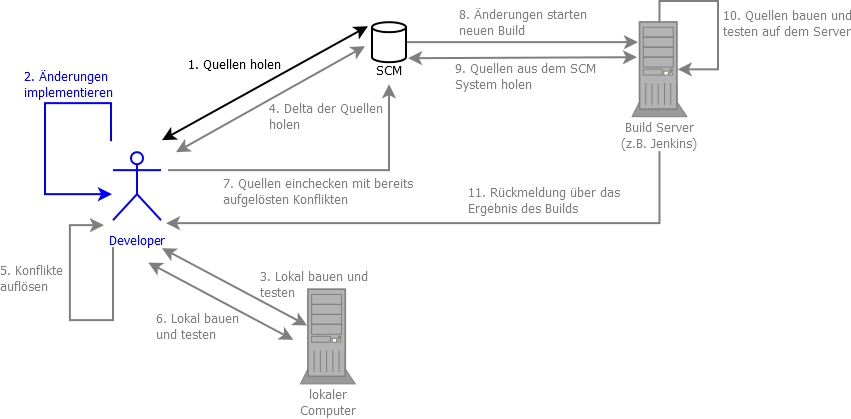
\includegraphics[width=110mm]{./Images/Schema-aufbau2.png}}	  
\end{figure}
\vspace{0.5cm} 
Die angestrebten Implementierungen werden durchgeführt
}
\only<3>{
\frametitle{Lokaler Build und Test}
\begin{figure}[h]
  \centering
  \fbox{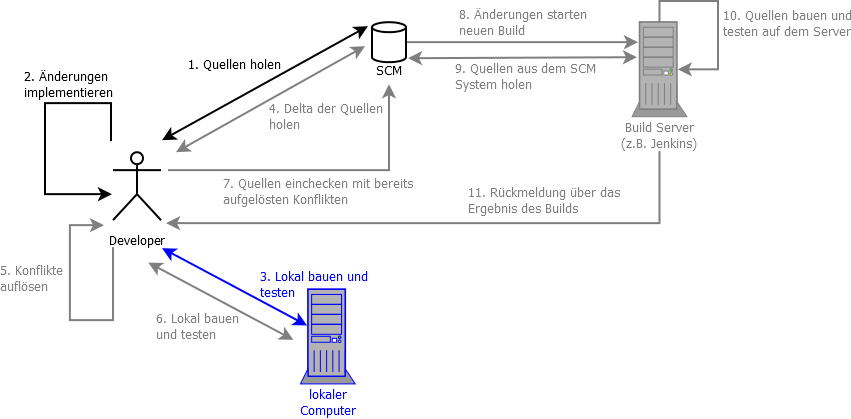
\includegraphics[width=110mm]{./Images/Schema-aufbau3.png}}	  
\end{figure}
\vspace{0.5cm} 
Lokaler Build mit Tests als erstes Quality Gate
}
\only<4>{
\frametitle{Source Code Delta holen}
\begin{figure}[h]
  \centering
  \fbox{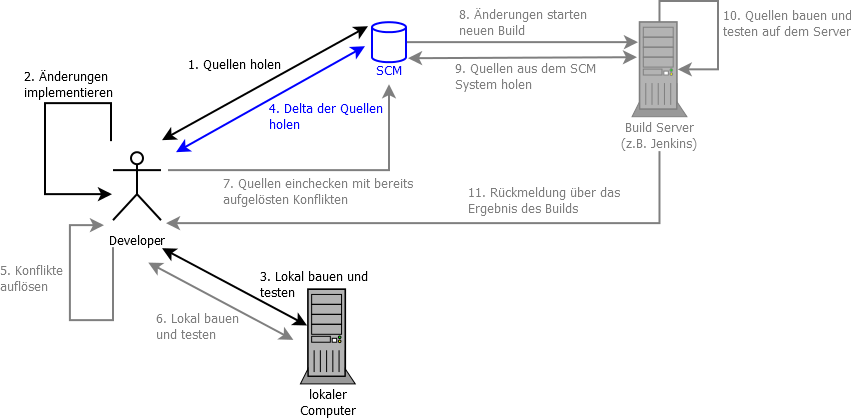
\includegraphics[width=110mm]{./Images/Schema-aufbau4.png}}	  
\end{figure}
\vspace{0.5cm} 
Zwischenzeitlich aufgelaufene Änderungen anderer Entwickler vom SCM holen
}
\only<5>{
\frametitle{Konflikte lösen}
\begin{figure}[h]
  \centering
  \fbox{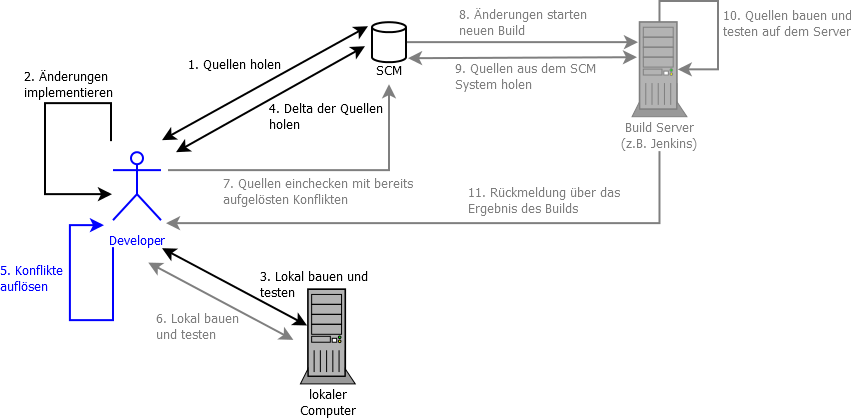
\includegraphics[width=110mm]{./Images/Schema-aufbau5.png}}	  
\end{figure}
\vspace{0.5cm} 
Neu entstandene Konflikte lokal auflösen
}
\only<6>{
\frametitle{Lokaler Build II}
\begin{figure}[h]
  \centering
  \fbox{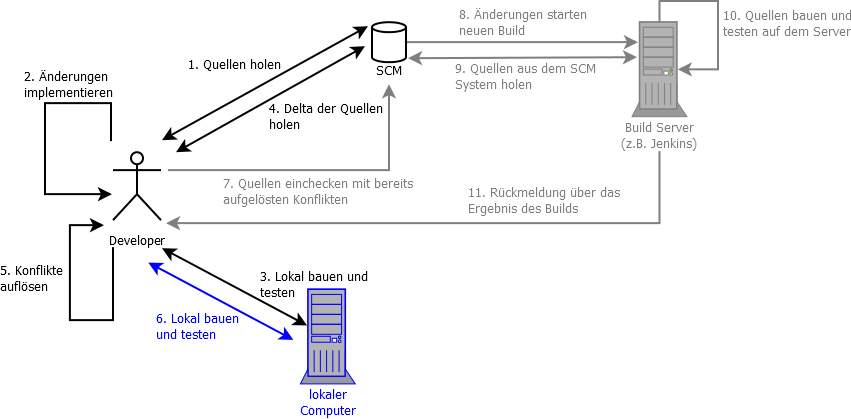
\includegraphics[width=110mm]{./Images/Schema-aufbau6.png}}	  
\end{figure}
\vspace{0.5cm} 
Lokaler Build mit Tests als letzes Quality Gate vor dem Checkin
}
\only<7>{
\frametitle{Checkin}
\begin{figure}[h]
  \centering
  \fbox{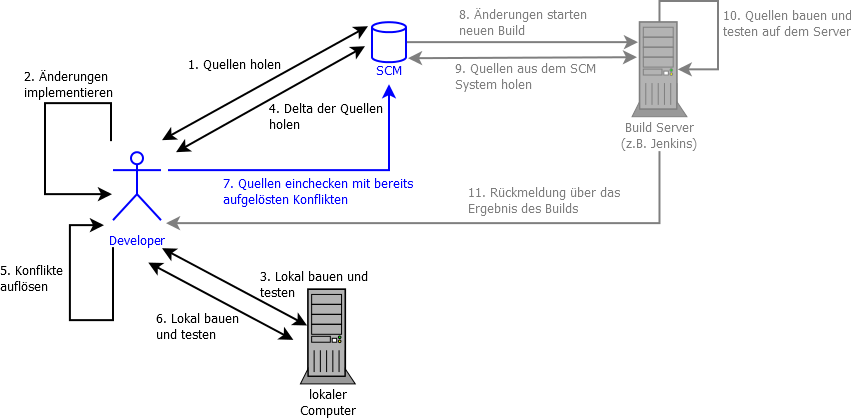
\includegraphics[width=110mm]{./Images/Schema-aufbau7.png}}	  
\end{figure}
\vspace{0.5cm} 
Nach erfolgreichem lokalen Build sind die Änderungen reif für den Checkin
}
\only<8>{
\frametitle{Trigger Build}
\begin{figure}[h]
  \centering
  \fbox{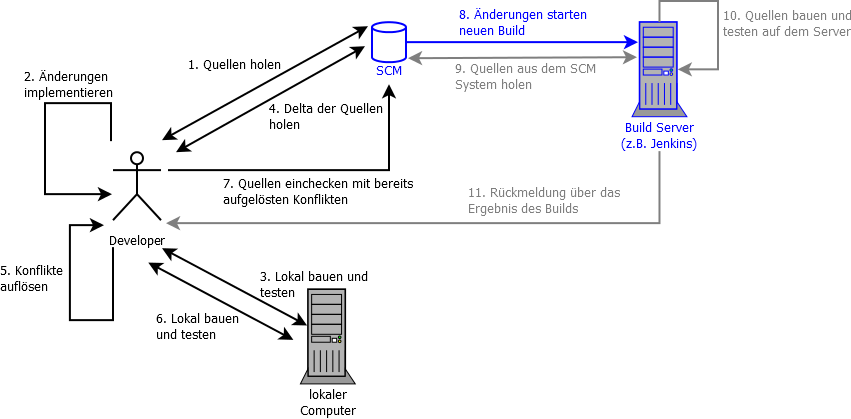
\includegraphics[width=110mm]{./Images/Schema-aufbau8.png}}	  
\end{figure}
\vspace{0.5cm} 
Ein automatischer Build startet, weil im SCM neue Sourcen vorhanden sind
}
\only<9>{
\frametitle{Aktuellen Stand holen}
\begin{figure}[h]
  \centering
  \fbox{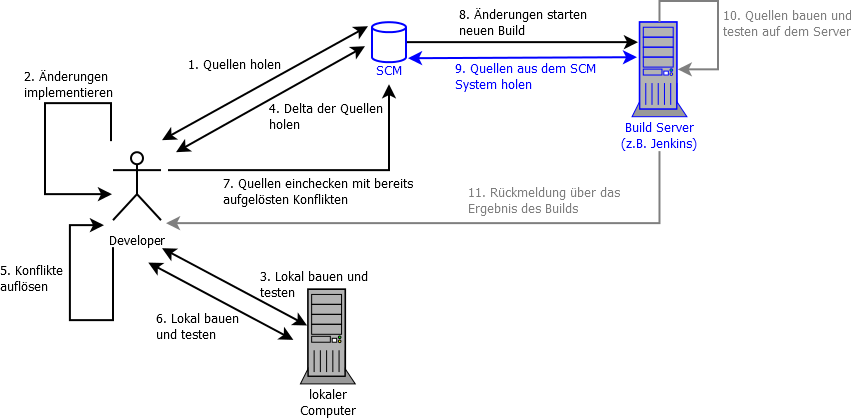
\includegraphics[width=110mm]{./Images/Schema-aufbau9.png}}	  
\end{figure}
\vspace{0.5cm} 
Der Build Server braucht die letzten Sourcen um sie zu bauen und zu testen
}
\only<10>{
\frametitle{Bauen am Server}
\begin{figure}[h]
  \centering
  \fbox{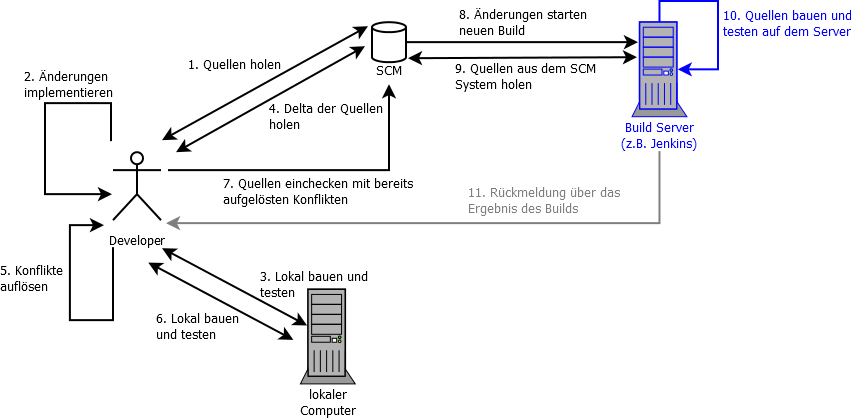
\includegraphics[width=110mm]{./Images/Schema-aufbau10.png}}	  
\end{figure}
\vspace{0.5cm} 
Der Server Build ist das ultimative Quality Gate im Prozess.\\
In diesem Schritt wird gebaut und getestet.
}
\only<11>{
\frametitle{Feedback}
\begin{figure}[h]
  \centering
  \fbox{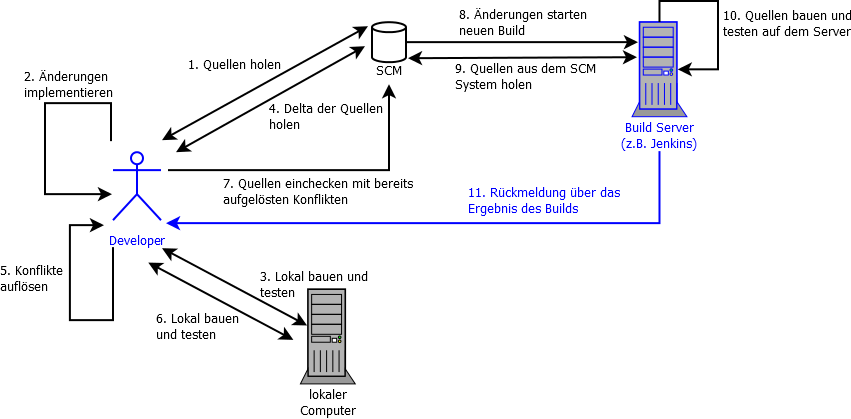
\includegraphics[width=110mm]{./Images/Schema-aufbau11.png}}	  
\end{figure}
\vspace{0.5cm} 
Das Ergebnis des Builds wird veröffentlicht und ruft eventuell weitere Aktionen des Entwicklers hervor.
}
\end{frame}



\iffalse
\subsection{Ablauf nach Martin Fowler}
\begin{frame} [t]
\frametitle{Baseline holen}
\begin{figure}[h]
  \centering
  \fbox{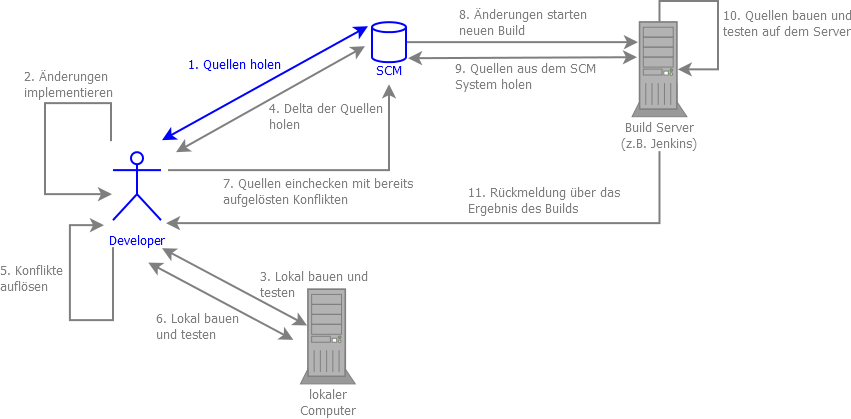
\includegraphics[width=110mm]{./Images/Schema-aufbau1.png}}	  
\end{figure}
\vspace{0.5cm} 
Entwickler holt sich Baseline
\end{frame}

\subsection{Ablauf nach Martin Fowler}
\begin{frame} [t]
\frametitle{Implementierung durchführen}
\begin{figure}[h]
  \centering
  \fbox{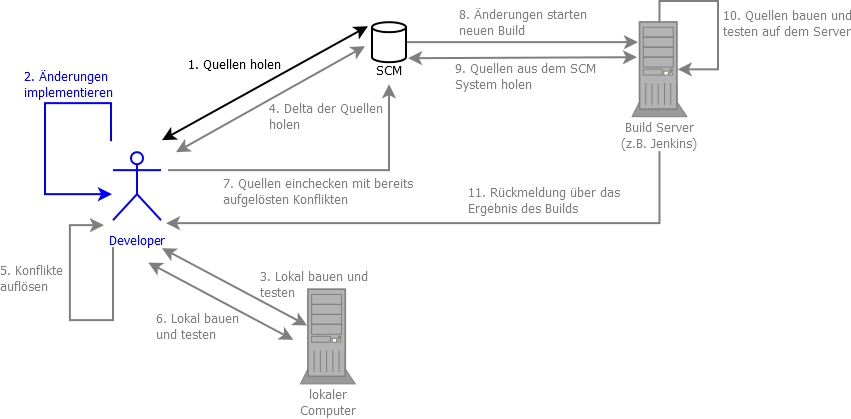
\includegraphics[width=110mm]{./Images/Schema-aufbau2.png}}	  
\end{figure}
\vspace{0.5cm} 
Die angestrebten Implementierungen werden durchgeführt
\end{frame}

\subsection{Ablauf nach Martin Fowler}
\begin{frame} [t]
\frametitle{Lokaler Build und Test}
\begin{figure}[h]
  \centering
  \fbox{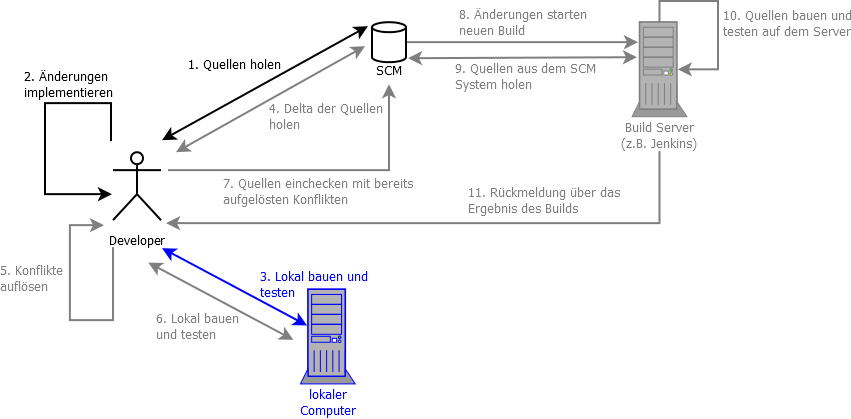
\includegraphics[width=110mm]{./Images/Schema-aufbau3.png}}	  
\end{figure}
\vspace{0.5cm} 
Lokaler Build mit Tests als erstes Quality Gate
\end{frame}

\subsection{Ablauf nach Martin Fowler}
\begin{frame} [t]
\frametitle{Source Code Delta holen}
\begin{figure}[h]
  \centering
  \fbox{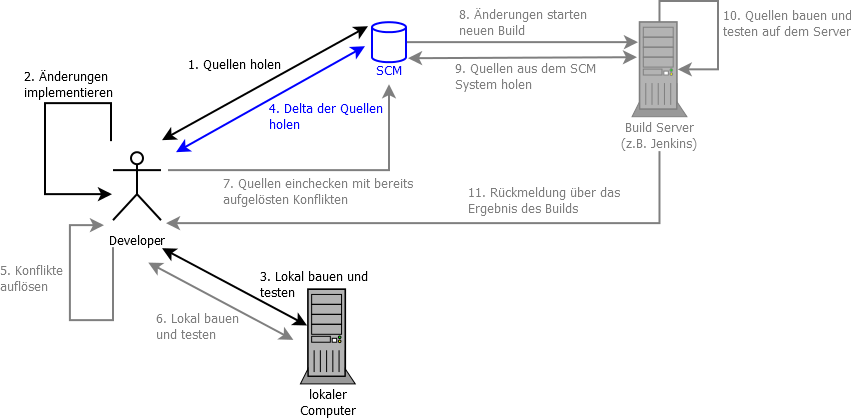
\includegraphics[width=110mm]{./Images/Schema-aufbau4.png}}	  
\end{figure}
\vspace{0.5cm} 
Zwischenzeitlich aufgelaufene Änderungen anderer Entwickler vom SCM holen
\end{frame}

\subsection{Ablauf nach Martin Fowler}
\begin{frame} [t]
\frametitle{Konflikte lösen}
\begin{figure}[h]
  \centering
  \fbox{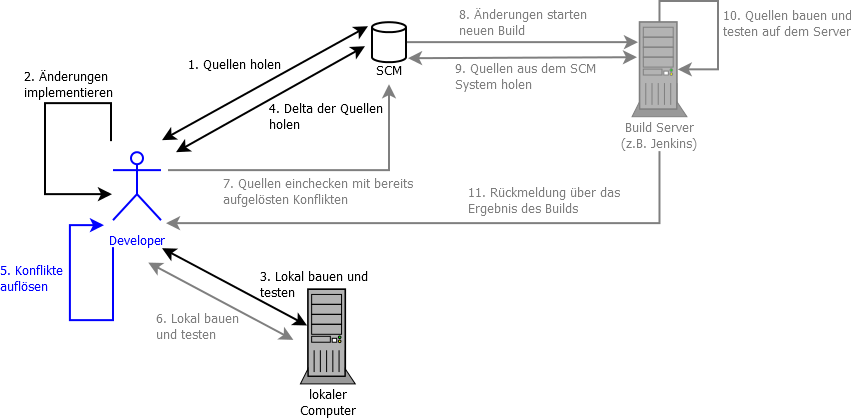
\includegraphics[width=110mm]{./Images/Schema-aufbau5.png}}	  
\end{figure}
\vspace{0.5cm} 
Neu entstandene Konflikte lokal auflösen
\end{frame}

\subsection{Ablauf nach Martin Fowler}
\begin{frame} [t]
\frametitle{Lokaler Build II}
\begin{figure}[h]
  \centering
  \fbox{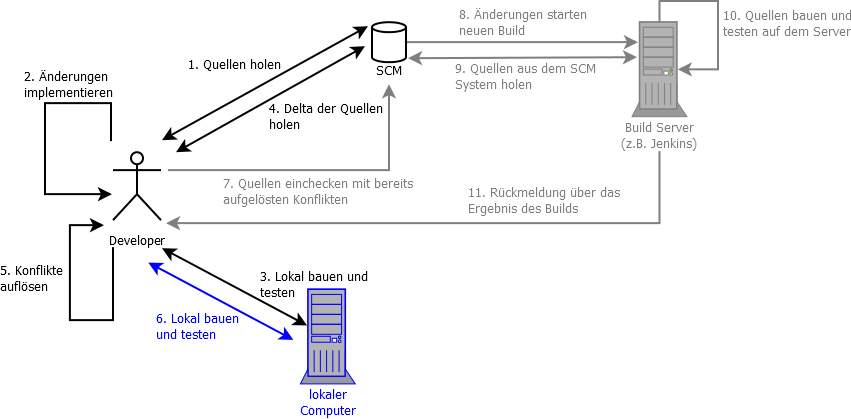
\includegraphics[width=110mm]{./Images/Schema-aufbau6.png}}	  
\end{figure}
\vspace{0.5cm} 
Lokaler Build mit Tests als letzes Quality Gate vor dem Checkin
\end{frame}

\subsection{Ablauf nach Martin Fowler}
\begin{frame} [t]
\frametitle{Checkin}
\begin{figure}[h]
  \centering
  \fbox{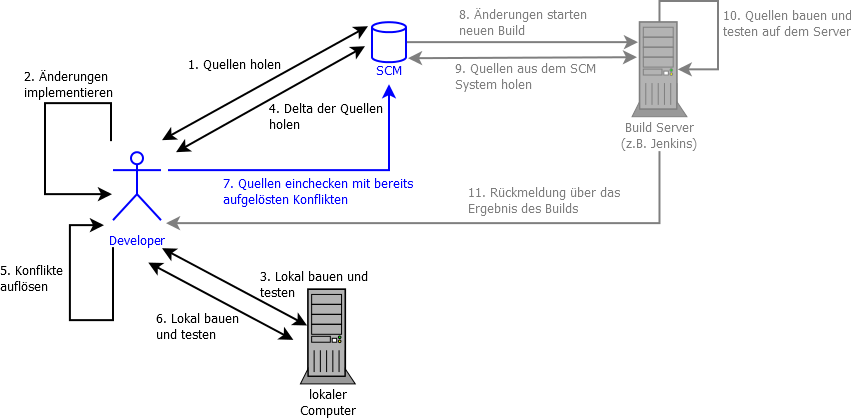
\includegraphics[width=110mm]{./Images/Schema-aufbau7.png}}	  
\end{figure}
\vspace{0.5cm} 
Nach erfolgreichem lokalen Build sind die Änderungen reif für den Checkin
\end{frame}

\subsection{Ablauf nach Martin Fowler}
\begin{frame} [t]
\frametitle{Trigger Build}
\begin{figure}[h]
  \centering
  \fbox{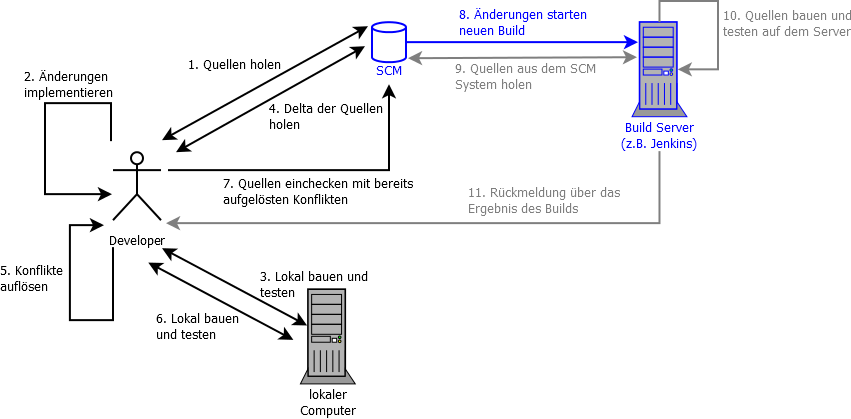
\includegraphics[width=110mm]{./Images/Schema-aufbau8.png}}	  
\end{figure}
\vspace{0.5cm} 
Ein automatischer Build startet, weil im SCM neue Sourcen vorhanden sind
\end{frame}

\subsection{Ablauf nach Martin Fowler}
\begin{frame} [t]
\frametitle{Aktuellen Stand holen}
\begin{figure}[h]
  \centering
  \fbox{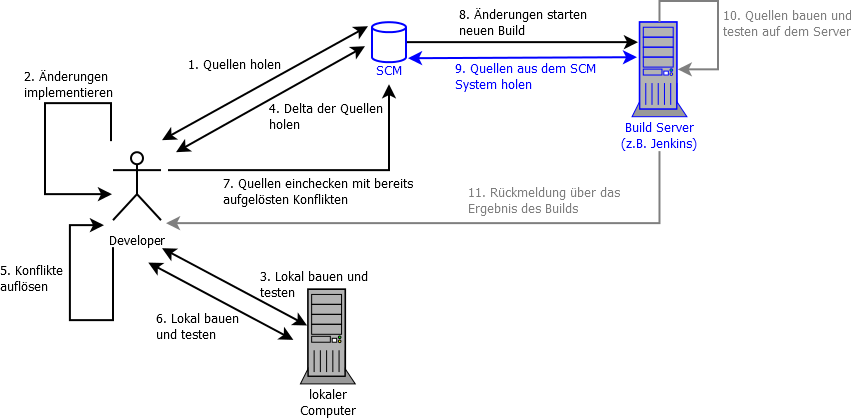
\includegraphics[width=110mm]{./Images/Schema-aufbau9.png}}	  
\end{figure}
\vspace{0.5cm} 
Der Build Server braucht die letzten Sourcen um sie zu bauen und zu testen
\end{frame}

\subsection{Ablauf nach Martin Fowler}
\begin{frame} [t]
\frametitle{Bauen am Server}
\begin{figure}[h]
  \centering
  \fbox{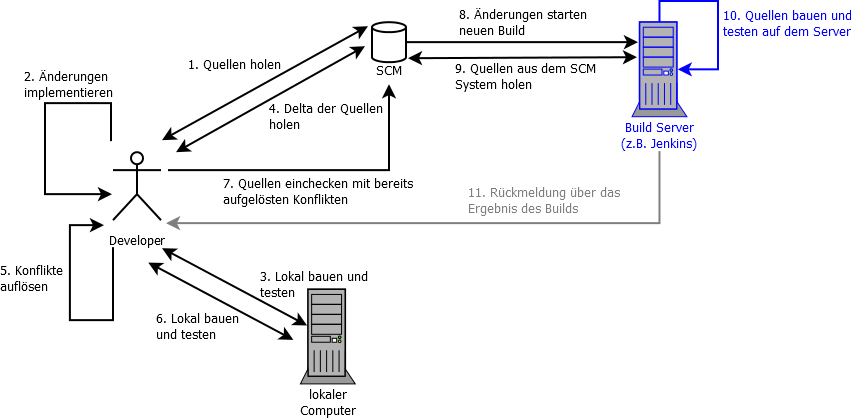
\includegraphics[width=110mm]{./Images/Schema-aufbau10.png}}	  
\end{figure}
\vspace{0.5cm} 
Der Server Build ist das ultimative Quality Gate im Prozess.\\
In diesem Schritt wird gebaut und getestet.
\end{frame}

\subsection{Ablauf nach Martin Fowler}
\begin{frame} [t]
\frametitle{Feedback}
\begin{figure}[h]
  \centering
  \fbox{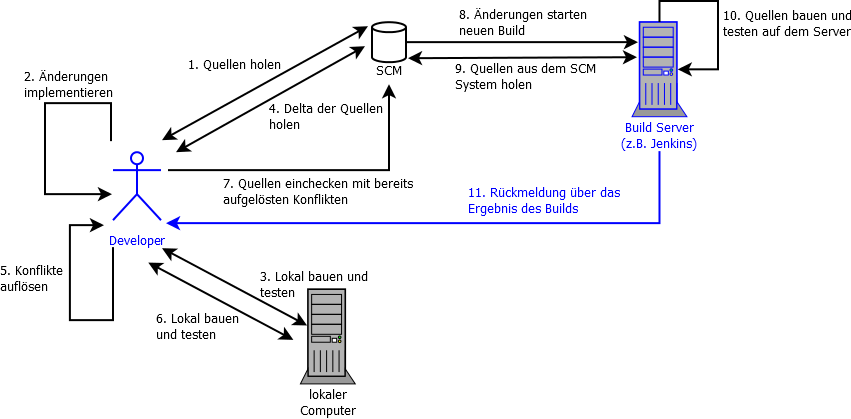
\includegraphics[width=110mm]{./Images/Schema-aufbau11.png}}	  
\end{figure}
\vspace{0.5cm} 
Das Ergebnis des Builds wird veröffentlicht und ruft eventuell weitere Aktionen des Entwicklers hervor.
\end{frame}
\fi
\section*{Vielen Dank}

\begin{frame} 
\frametitle{Vielen Dank}

\begin{center}
\Huge{Vielen Dank für Ihre Aufmerksamkeit!}
\end{center}

\end{frame}




\end{document}